\documentclass[tikz]{standalone}

\usepackage{fontspec}

\usetikzlibrary{arrows}
\usetikzlibrary{calc}
\usetikzlibrary{decorations.pathreplacing}
\usetikzlibrary{positioning}
\usetikzlibrary{matrix}

\usepackage{fontspec}

\begin{document}

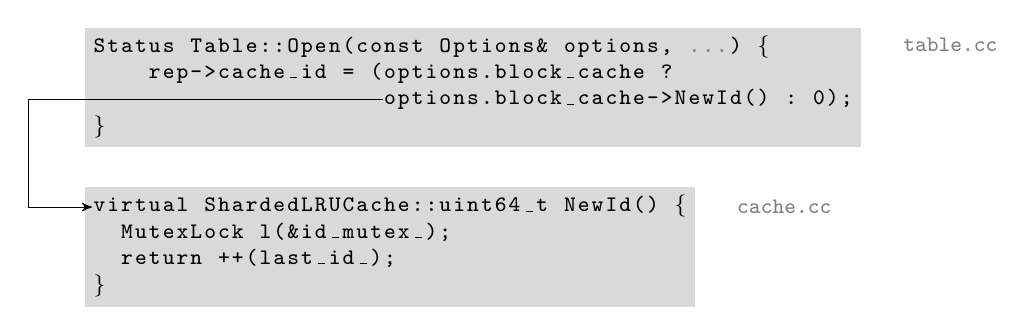
\begin{tikzpicture}
  [node distance=5mm, >=stealth',
  every node/.style={font=\footnotesize},
  every matrix/.style={fill=black!15, inner sep=1mm, row sep=0.5mm,
                        matrix of nodes, nodes in empty cells,
                        minimum height=0.5em, minimum width=.5em,
                        nodes={anchor=base, inner sep=0, font=\ttfamily\footnotesize}}]

  \matrix (Open) {
S & t & a & t & u & s &   & T & a & b & l & e & : & : & O & p & e & n & ( & c & o & n & s & t &   & O & p & t & i & o & n & s & \& &   & o & p & t & i & o & n & s & , &   & |[black!50]|. & |[black!50]|. & |[black!50]|. & ) &   & \{ &   &   &   &   &   &   \\
  &   &   &   & r & e & p & - & > & c & a & c & h & e & \_ & i & d &   & = &   & ( & o & p & t & i & o & n & s & . & b & l & o & c & k & \_ & c & a & c & h & e &   & ? &   &   &   &   &   &   &   &   &   &   &   &   &   \\
  &   &   &   &   &   &   &   &   &   &   &   &   &   &   &   &   &   &   &   &   & o & p & t & i & o & n & s & . & b & l & o & c & k & \_ & c & a & c & h & e & - & > & N & e & w & I & d & ( & ) &   & : &   & 0 & ) & ; \\
\} &   &   &   &   &   &   &   &   &   &   &   &   &   &   &   &   &   &   &   &   &   &   &   &   &   &   &   &   &   &   &   &   &   &   &   &   &   &   &   &   &   &   &   &   &   &   &   &   &   &   &   &   &   &   \\
  };

  \matrix [below=of Open.south west, anchor=north west] (NewId) {
v & i & r & t & u & a & l &   & S & h & a & r & d & e & d & L & R & U & C & a & c & h & e & : & : & u & i & n & t & 6 & 4 & \_ & t &   & N & e & w & I & d & ( & ) &   & \{ \\
  &   & M & u & t & e & x & L & o & c & k &   & l & ( & \& & i & d & \_ & m & u & t & e & x & \_ & ) & ; &   &   &   &   &   &   &   &   &   &   &   &   &   &   &   &   &   \\
  &   & r & e & t & u & r & n &   & + & + & ( & l & a & s & t & \_ & i & d & \_ & ) & ; &   &   &   &   &   &   &   &   &   &   &   &   &   &   &   &   &   &   &   &   &   \\
\} &   &   &   &   &   &   &   &   &   &   &   &   &   &   &   &   &   &   &   &   &   &   &   &   &   &   &   &   &   &   &   &   &   &   &   &   &   &   &   &   &   &   \\
  };

 \node [above, anchor=west, black!50, xshift=0.5cm]
        at (Open-1-55.north east)
        {\texttt{table.cc}};

 \node [above, anchor=west, black!50, xshift=0.5cm]
        at (NewId-1-43.east)
        {\texttt{cache.cc}};

  \draw [->] let \p1 = (Open-3-22.west),
                 \p2 = (NewId-1-1.west)
              in (\p1) -- ++(-4.5cm, 0) -- (\x1 - 4.5cm, \y2) -- (\p2);
\end{tikzpicture}

\end{document}
